\documentclass[12pt]{article}
\usepackage[french]{babel}
\usepackage{natbib}
\usepackage{url}
\usepackage[utf8x]{inputenc}
\usepackage{amsmath}
\usepackage{graphicx}
\usepackage[svgnames]{xcolor}
\usepackage{vmargin}
\setmarginsrb{3 cm}{1 cm}{3 cm}{1.5 cm}{1 cm}{0.5 cm}{1 cm}{1.5 cm}
\usepackage{multirow}
\graphicspath{{images/}}
\usepackage{parskip}
\usepackage{fancyhdr}
\usepackage[T1]{fontenc}
\usepackage{url}
\usepackage{pdfpages}
\usepackage{url}
\usepackage{hyperref}
\usepackage{graphicx}
\usepackage{subfigure}
\usepackage{caption}
\usepackage{subcaption}
\usepackage{empheq, cases}
\usepackage{amssymb}
\usepackage{amsmath}
\usepackage{verbatimbox}
\usepackage{tcolorbox}
\usepackage{float}
\usepackage{multicol}
\usepackage[compact]{titlesec}
\usepackage[colorinlistoftodos]{todonotes}
\usepackage{sectsty}

\xdefinecolor{gray}{named}{lightgray}
\xdefinecolor{alice}{named}{AliceBlue}
\xdefinecolor{saumon}{named}{PeachPuff}
\definecolor{myred1}{RGB}{255, 0, 0}
\definecolor{mygreen1}{RGB}{0, 126, 0}
\definecolor{myblue1}{RGB}{0, 0, 61}
\definecolor{lightgray}{rgb}{0.83, 0.83, 0.83}
\definecolor{brick}{rgb}{0, 0, 0.50}
\sectionfont{\color{brick}}  % sets colour of chapters
\subsectionfont{\color{RoyalBlue}}

\tcbset{colback=lightgray,colframe=black}



\title{\color{brick} Optimisation TD 4:\\
\LARGE{Recuit simulé et le voyageur de commerce}}								% Title
\author{Émilie Mathian}								% Author
\date{Année 2018 - 2019}											% Date

\makeatletter
\let\thetitle\@title
\let\theauthor\@author
\let\thedate\@date
\makeatother

\pagestyle{fancy}
\fancyhf{}
\rhead{\theauthor}
\lhead{Optimisation TD 1}
\cfoot{\thepage}
%%%%%%%%%%%%%%%%%%%%%%%%%%%%%%%%%%%%%%%%%%%%%%%%%%%%%%%%%%%%%%%
\usepackage{eso-pic}
\newcommand\BackgroundPic{%
\put(0,0){%
\parbox[b][\paperheight]{\paperwidth}{%
\vfill
\centering
\includegraphics[width=\paperwidth,height=\paperheight,%
keepaspectratio]{background.png}%
\vfill
}}}
  
  
\begin{document}

%%%%%%%%%%%%%%%%%%%%%%%%%%%%%%%%%%%%%%%%%%%%%%%%%%%%%%%%%%%%%%%%%%%%%%%%%%%%%%%%%%%%%%%%%

\begin{titlepage}
	\centering
    \vspace*{0.5 cm}
    \vspace{-3.5cm}
    
\includegraphics[width = 4cm]{logo.png}\\	% University Logo
    \textsc{\LARGE Institut National des Sciences Appliquées de Lyon}\\[2.0 cm]	% University Name
	\textsc{\Large $4^{eme}$ Année Bioinformatique et Modélisation}\\[0.5 cm]				% Course Code
	\textsc{\large Professeur: Noëlie DEBS }\\[0.5 cm]				% Course Name
	\rule{\linewidth}{0.2 mm} \\[0.4 cm]
	{ \huge \bfseries \thetitle}\\
	\rule{\linewidth}{0.2 mm} \\[1.5 cm]
	
	\begin{minipage}{0.4\textwidth}
		\begin{flushleft} \large
			\emph{Auteur:}
			\theauthor
			\end{flushleft}
			\end{minipage}~
			\begin{minipage}{0.4\textwidth}	
	\end{minipage}\\[2 cm]
    \vspace{-1.8cm}
	 \begin{figure}[H]
	\begin{center}
	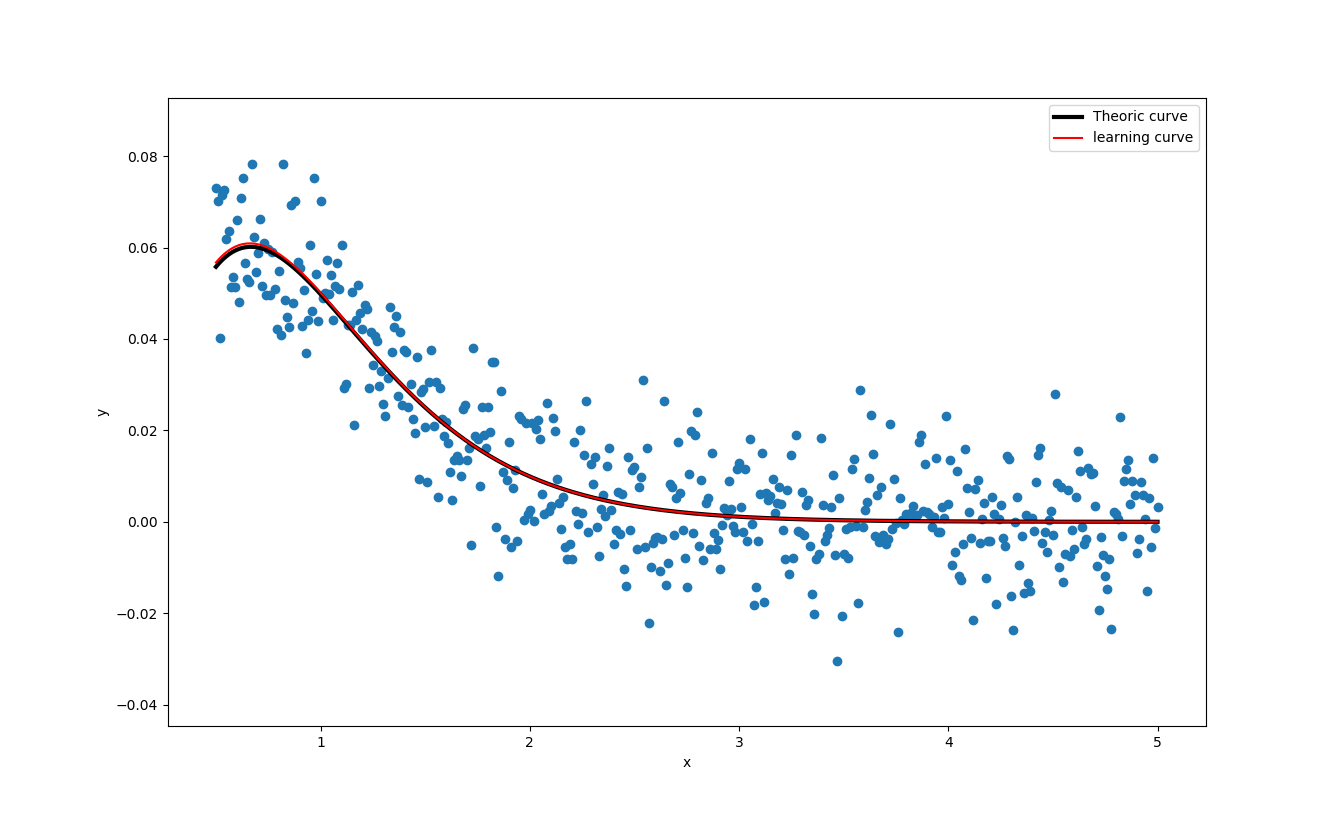
\includegraphics[width=0.9 \textwidth]{Figure_1.png}
\end{center}
\end{figure}

	{\large \thedate}\\[1 cm]
    
	\vfill

 

\end{titlepage}
\pagebreak
%%%%%%%%%%%%%%%%%%%%%%%%%%%%%%%%%%%%%%%%%%%%%%%%%%%%%%%%%%%%%%%%%%%%%%%%%%%%%%%%%%



\newpage 

\tableofcontents

\newpage

\section{Le recuit simulé}
\begin{center}
\fcolorbox{black}{lightgray}{
\begin{minipage}{\linewidth}
\textbf{Problématique :} \\
Le recuit simulé est un algorithme d'optimisation intégrant une part d'aléatoire. Cet algorithme est une analogie à une technique employée en métallurgie, où la fonction à minimiser est l'énergie libre d'un système. On voudrait ainsi obtenir un métal ayant la plus grande stabilité soit un cristal, or cet état n'est atteint que lorsque le processus de refroidissement est lents, sinon on risque d'obtenir un polycristal de plus haute énergie libre. Nous étudierons  ainsi l'effet du 'refroidissement'. De plus par analogie à la thermodynamique, si l'on considère un système à l'équilibre à une température T, ce système a une probabilité faible de changer d'état et cette probabilité décroît avec T (probabilité de Boltzmann). Nous observerons l'importance de cette loi qui donne de la souplesse à l'algorithme.\\
Le rapport suivant reprend le programme \textit{'recuit.py'}.
\end{minipage}}
\end{center}


\subsection{Fonction de $\mathbb{R}$ dans $\mathbb{R}$}
\begin{minipage}{0.5\textwidth}

\textbf{\color{brick}1.} 
D'après la représentation de la fonction $f(x)$ \textbf{[\ref{Q1}}, nous observons l'existence d'un minimum local et d'un global, et d'un maximum local. Nous pouvons numéiquement estimer les coordonnées de ces points d'inflexion. Le minimum local est atteint pour $x\simeq 2.823$ alors $f(2.823)\simeq -114.55$, le maximum local est atteint pour $x\simeq0.024$ alors $f(0.024)\simeq 1.012$ et enfin le minimum global est atteitn pout $x\simeq 3.548$ et alors $f(3.548)\simeq -133.41$.
\end{minipage} \hfill
\begin{minipage}{0.45\textwidth}
\begin{figure}[H]
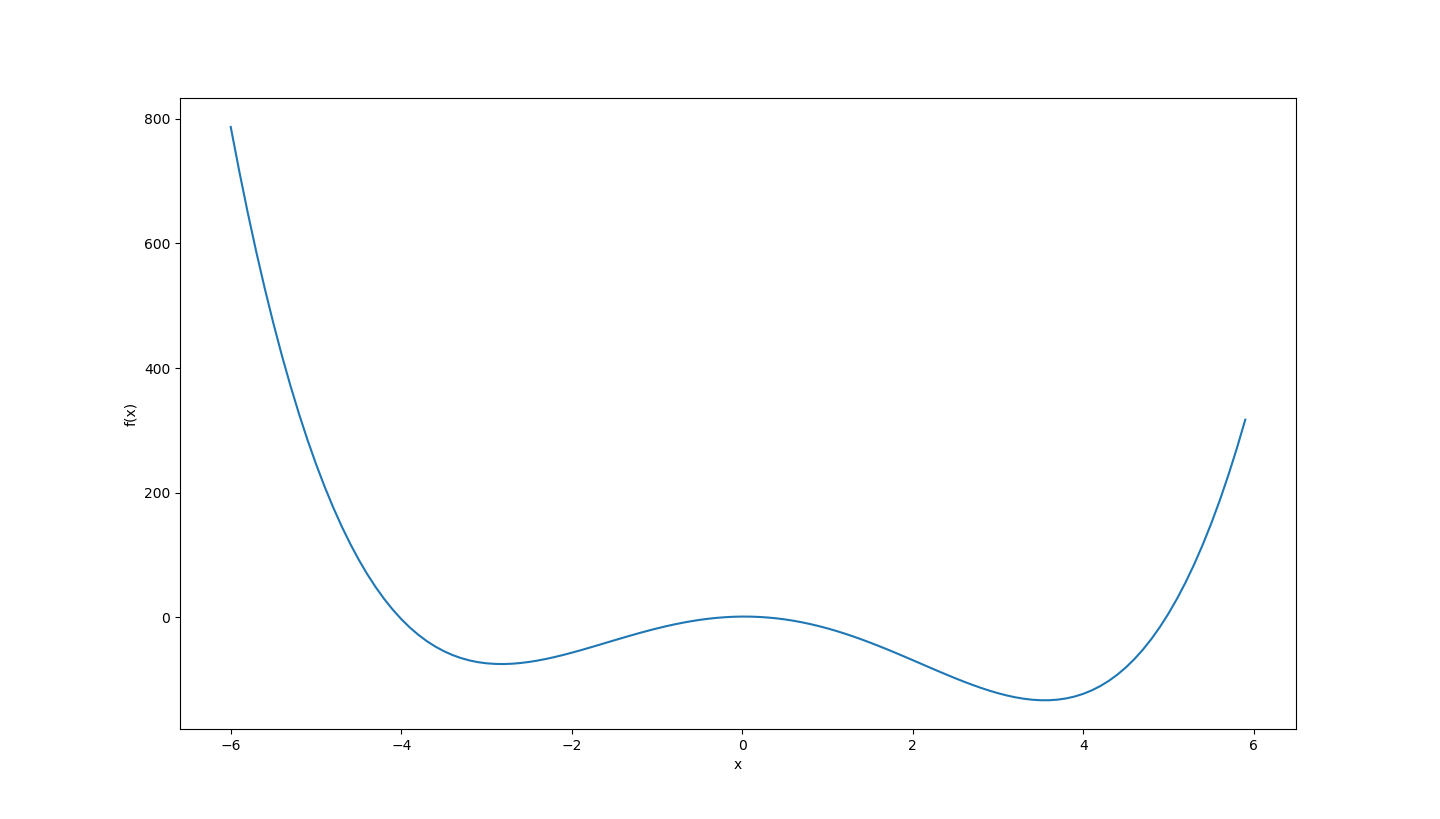
\includegraphics[width=1\textwidth]{Q1.png}
\caption{Représentation de la fonction à minimiser  $f(x)=x^4 - x^3 -20x^2+x+1$}
\label{Q1}
\end{figure}
\end{minipage}


\begin{minipage}{0.5\textwidth}
\textbf{\color{brick}2.} L'implémentation de la méthode du recuit simulé pour la fonction $f$ décrite ci-dessus fait référence à la fonction \verb|recuit_f1| (cf : \verb|recuit.py|).\\
 Pour tester notre algorithme nous prenons les conditions suivantes : $k=10$, $k'=0.5$, $T=1/t$ et $t_{max}=1$, la solution obtenue est illustrée ci-contre \textbf{[\ref{Q1_2}]}. Nous remarquons que la solution converge vers le minimum global, avec comme résultat final $x_{t=10000} \simeq 3.548  $ et $f(x_{t=10000}) \simeq -133.41$. En revanche l'algorithme a parcouru un vaste espace et des valeurs très éloignées de la solution avant de cnverger.
\end{minipage} \hfill
\begin{minipage}{0.45\textwidth}
\begin{figure}[H]
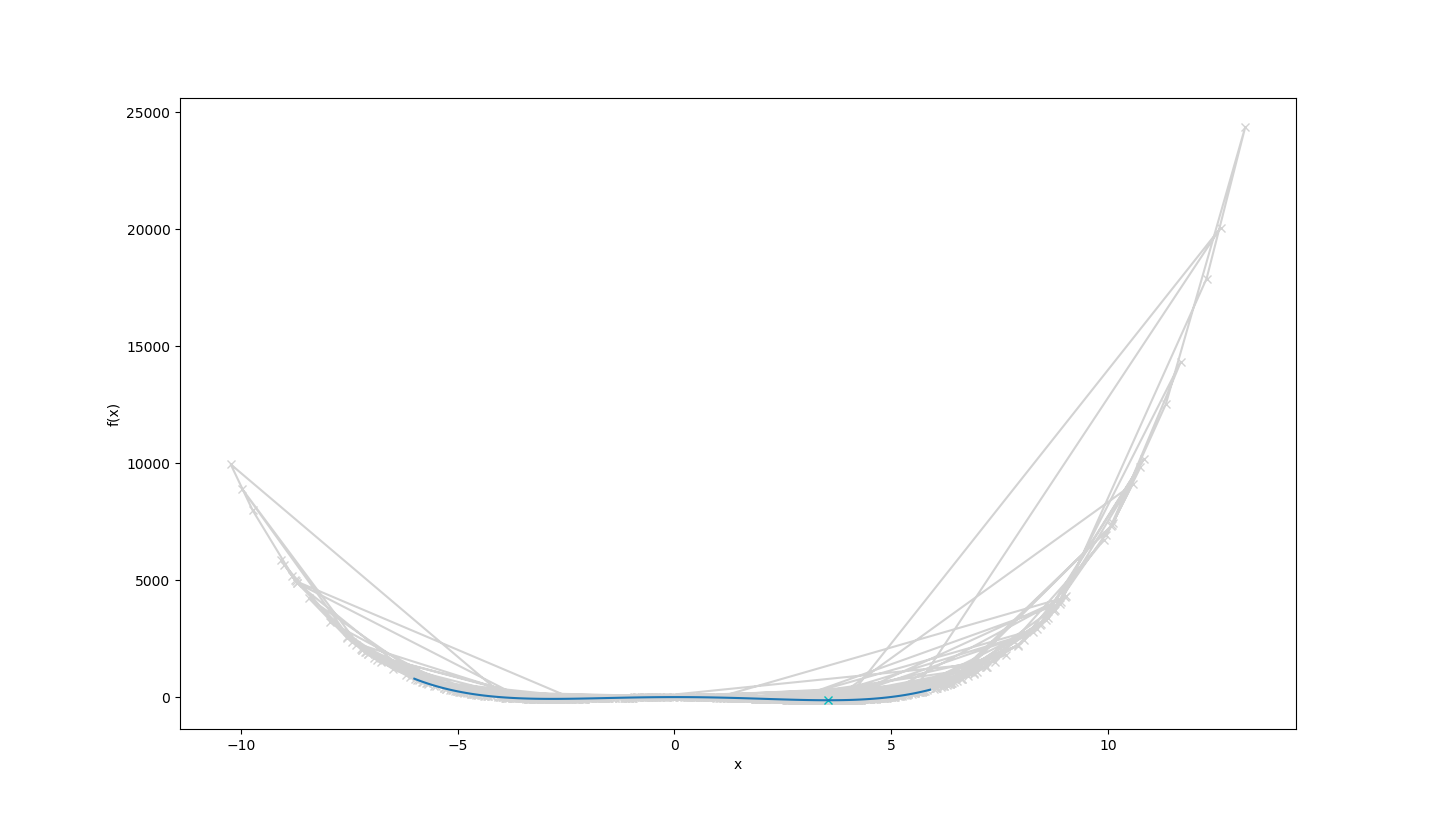
\includegraphics[width=1\textwidth]{Q1_2.png}
\caption{Représentation de la fonction à minimiser  $f$, du parcours de l'algorithme du recuit simulé et de la solution finale retenue.}
\label{Q1_2}
\end{figure}
\end{minipage}

\begin{figure}[H]
  \centering
  \subfigure[Variation de k]{%
    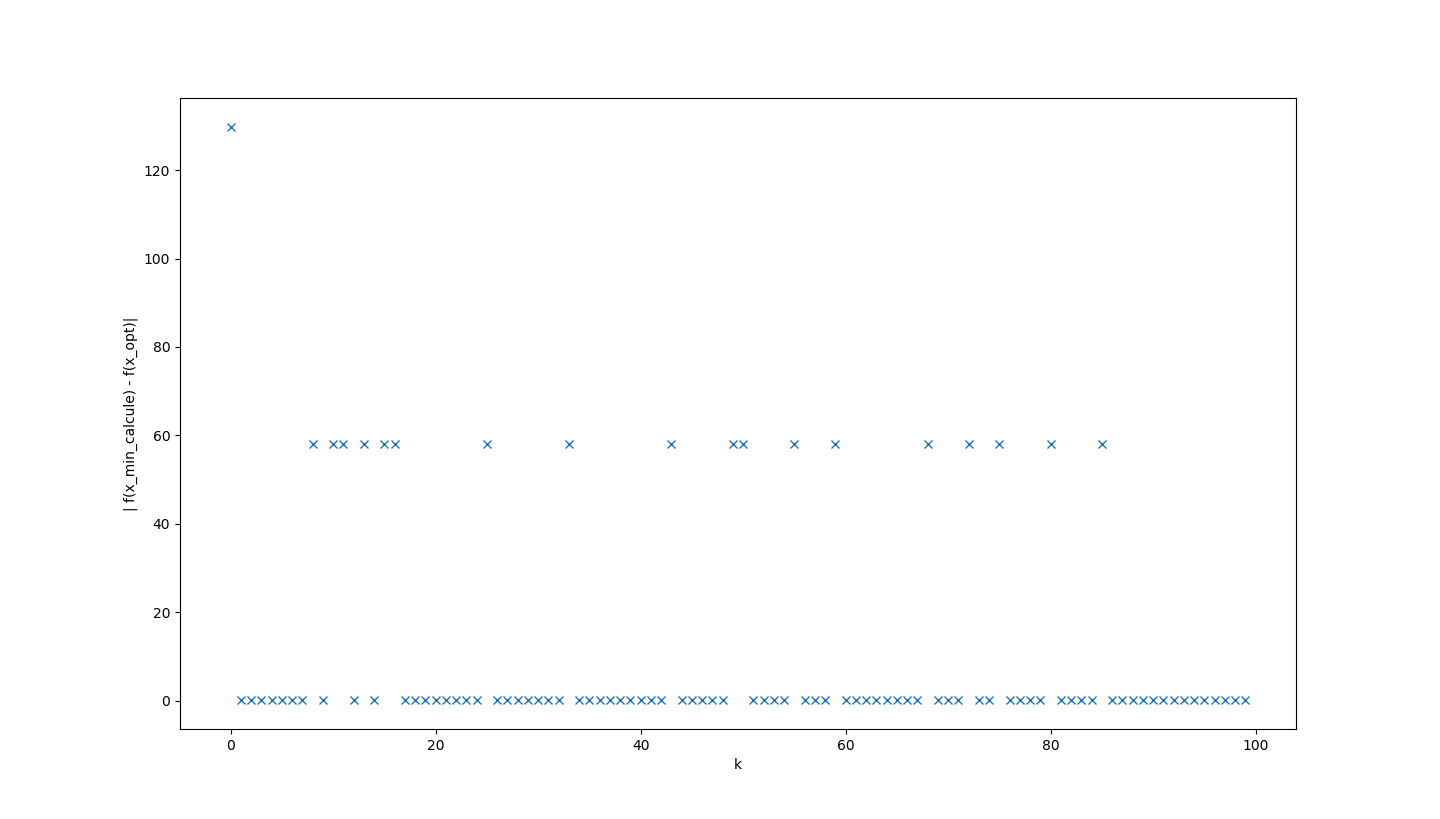
\includegraphics[width=0.45\textwidth]{Q1_k.png}
    \label{fig:a}%
    }%or more
    \subfigure[Variation de k']{%
    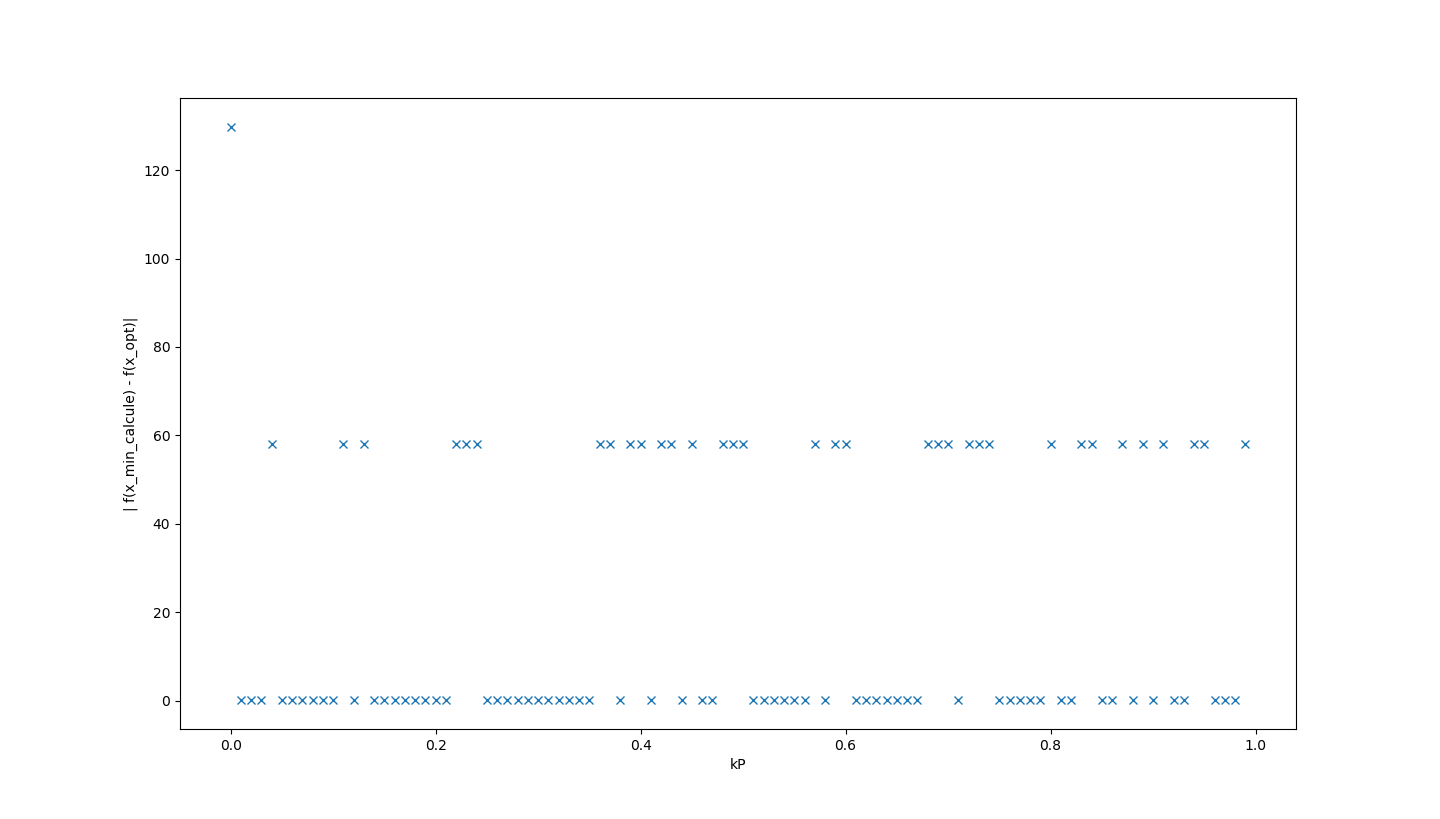
\includegraphics[width=0.45\textwidth]{Q1_kp.png}
    \label{fig:b}%
  }%  
  \caption{Étude de l'écart entre la solution calculée et la solution analytique pour 10000 itération avec $x_0 = 0.5$, et pour \textbf{a} $kp=0.5$ et $k\in [0,30]$ et  pour \textbf{b} $kp \in [0,1]$ et $k= 10$}
  \label{fig:ab}
\end{figure}
D'après la figure \textbf{[\ref{fig:a}]}, on observe que l'algorithme converge plus fréquemment vers le minimum local lorsque k est faible, la densité du nuage de point, pour $f(\hat{x_opt}- f(x_opt)) \simeq 60$ , est plus forte à gauche. Ainsi plus on permet à l'algorithme d'inspecter un voisinage éloigné du $x$ courant plus  la probabilité de trouver le minimum global croit.  À l'inverse d'après la figure \textbf{[\ref{fig:b}]} plus $k'$ augmente (noté kp) augmente plus la probabilité de converger vers le minimum local augmente, la densité du nuage de point pour  $f(\hat{x_opt}- f(x_opt)) \simeq 60$ , est plus forte à droite. Ainsi plus on abaisse la probabilité d'accepter un point qui augmentait localement le coût plus la probabilité de converger vers le minimum global croît. Néanmoins ces remarques semblent approximatives et pourraient être dues au hasard.//
C'est pourquoi nous allons tenter de mettre en place un test statistique pour savoir si le nombre de succès de l'algorithme (convergence vers le minimum global) est fonction des paramètres $k$ ou $kp$. Pour cela nous choisissons de séparer les valeurs du paramètre  testées en deux échantillons et ainsi d'établir les hypothèse suivantes :
\begin{align*}
    H_O : \quad S_{k<m} &=  S_{k>m} \\
    H_1 : \quad S_{k>m} &>  S_{k>m}
\end{align*}

Pour réaliser ce test nous générons 15 simulations ou nous faisons varier le paramètre, pour chaque simulation nous retenons la proportion de succès dans chacune des deux parties soit pour $k<1m$ et pour $k>m$. Puis par un test de Student unilatéral pour comparer les moyennes des échantillons simulés. Nous calculons la valeur de T tel que $$T = \frac{\Bar{S_{k>15} - \Bar{S_{k<m}}}}{\sqrt{\frac{s'^2_{k>m}}{n_1} + \frac{s'^2_{k<m}}{n_2}}    }$$
Nous obtiendrons ensuite la pvalue grâce à la librairie \verb|scipy.stats.t|.

% Résultat du test  k 
\begin{scriptsize}
\begin{verbatim}
# Paramètres à tester k:
> K = seq(0,15,0.5)  k' moy = 0.7.5   
> Nombre de k testé :  n_inf = 30 ; n_sup = 30
# Paramètres de la simulation : 
> Nombre de répétition : n = 40
> k' = 0.5 , tmax = 10000, x0 = random.unif(-5,5)
# Définition du test :
> H0 : Nb_succès_moyen | k <7.5 = Nb_succès_moyen | k >7.5 
> H1 : Nb_succès_moyen | k <7.5 < Nb_succès_moyen | k >7.5 
# Résultats :
> Stat_t = 2.629
> P_value = 5e-3
# Conclusion : On rejette H0 au risque 5\%
\end{verbatim}
\end{scriptsize}
\\
\begin{scriptsize}
\begin{verbatim}
# Paramètres à tester k':
> K' = seq(0,0.5,0.02)  k' moy = 0.25   
> Nombre de k testé :  n_inf = 25 ; n_sup = 25
# Paramètres de la simulation : 
> Nombre de répétition : n = 40
> k = 10 , tmax = 10000, x0 = random.unif(-5,5)
# Définition du test :
> H0 : Nb_succès_moyen | k <0.25 = Nb_succès_moyen | k >0.25 
> H1 : Nb_succès_moyen | k <0.25 > Nb_succès_moyen | k >0.25 
# Résultats :
> Stat_t = 2.269
> P_value = 0.012
# Conclusion : On rejette H0 au risque 5\%
\end{verbatim}
\end{scriptsize}

Ces conclusions sont vrais si on s'interesse sur l'intervalle $k'\in[0,05]$, en effet si on réalise ce test sur $[0,1]$ la différence de moyennes n'est plus significatives !

\begin{minipage}{0.5\textwidth}
D'après la figure \textbf{[\ref{Q1_T}]}, nous observons que si le nombre d'itération est trop faible $t_{max}<1500$ l'algorithme n'a pa le 'temps' de converger si $t_{max}$ est supérieur à ce seuil alors l'algorithme convergera vers l'un des deux minimums.
\end{minipage} \hfill
\begin{minipage}{0.45\textwidth}
\begin{figure}[H]
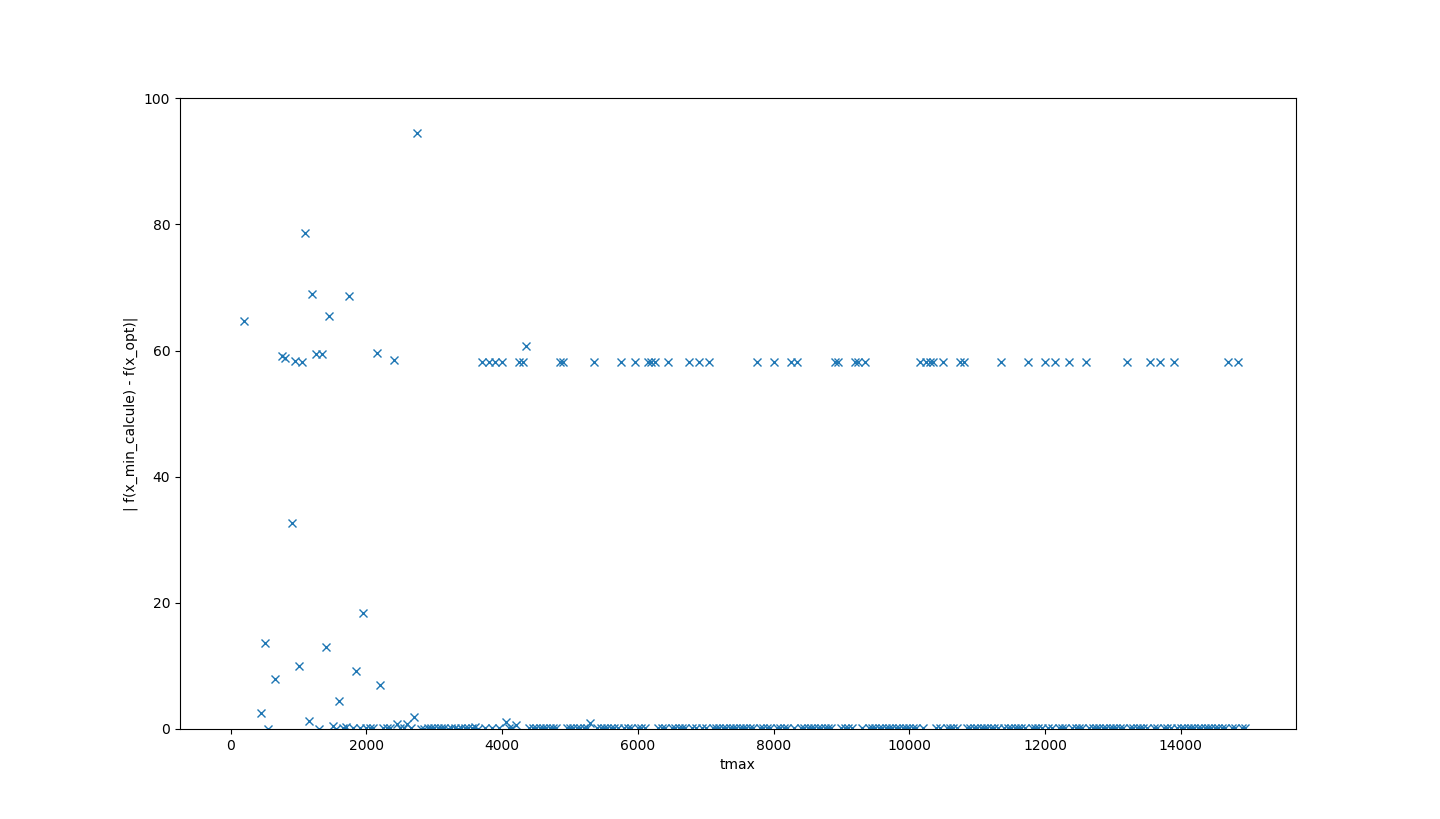
\includegraphics[width=1\textwidth]{Q1_T.png}
\caption{valeur absolue de l'erreur en fonction du nombre d'itération maximal}
\label{Q1_T}
\end{figure}
\end{minipage}



\begin{minipage}{0.5\textwidth}
Rappelons que le choix du nombre d'itérations maximale influence également la température étant donnée que $T=\frac{1}{t}$, pour observer l'influence de la température nous pouvons faire varier le coefficient  '1000' pour ralentir ou augmenter le processus de refroidissement. Nous faisons donc varier ce coefficient entre $[0,2000]$ et nous obtenons les résultats ...
% Ref image
\end{minipage} \hfill
\begin{minipage}{0.45\textwidth}
\begin{figure}[H]
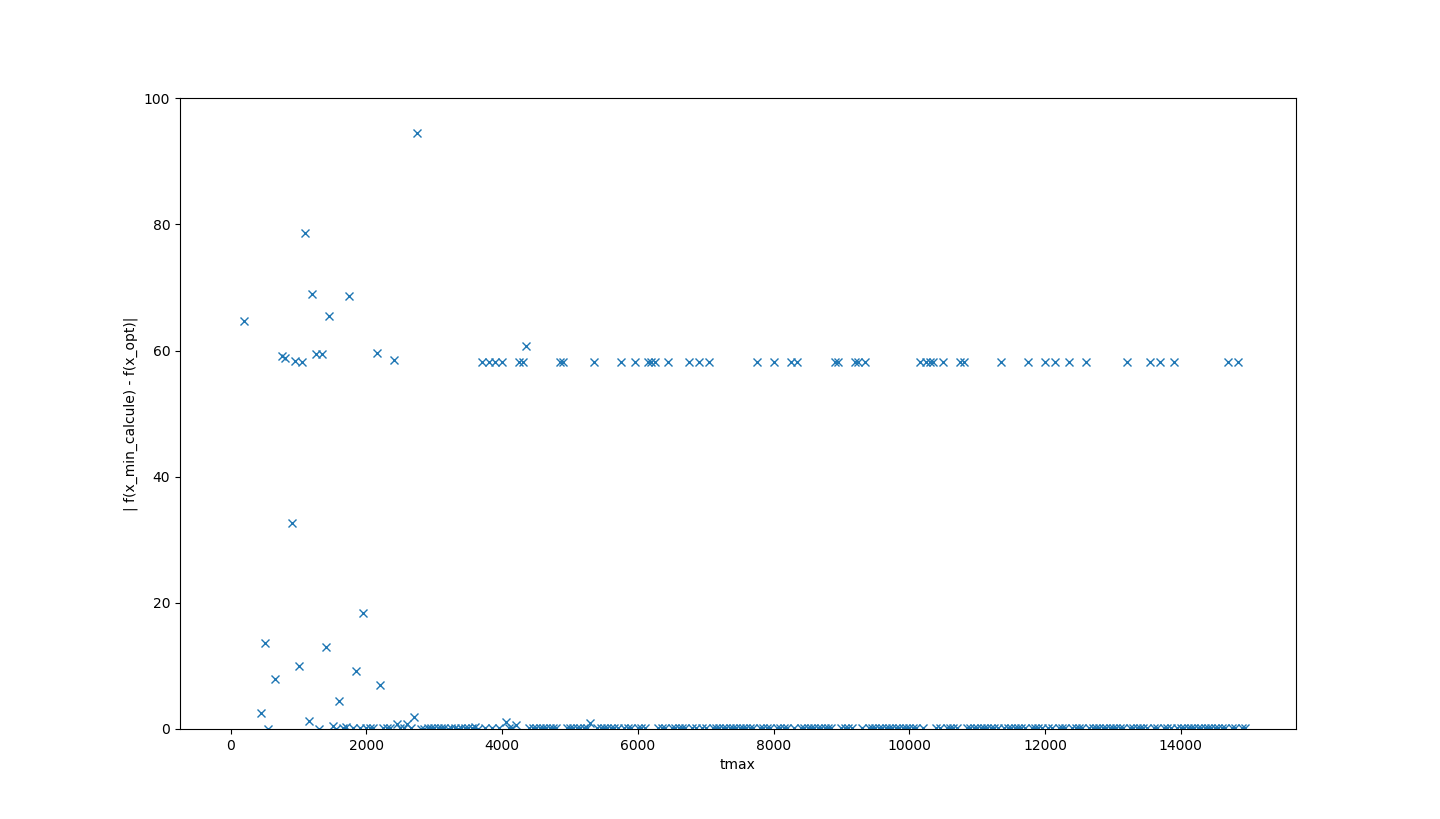
\includegraphics[width=1\textwidth]{Q1_T.png}
\caption{valeur absolue de l'erreur en fonction du nombre d'itération maximal}
\label{Q1_T}
\end{figure}
\end{minipage}

\textbf{\color{brick}3.} D'après les analyses précédentes pour augmenter la convergence de l'algorithme vers le minimum global nous choisissons $k=20$, $k'p=0.1$ et $t_{max}=15000$, nous obtenons alors les résultats suivants:
\begin{figure}[H]
\centering
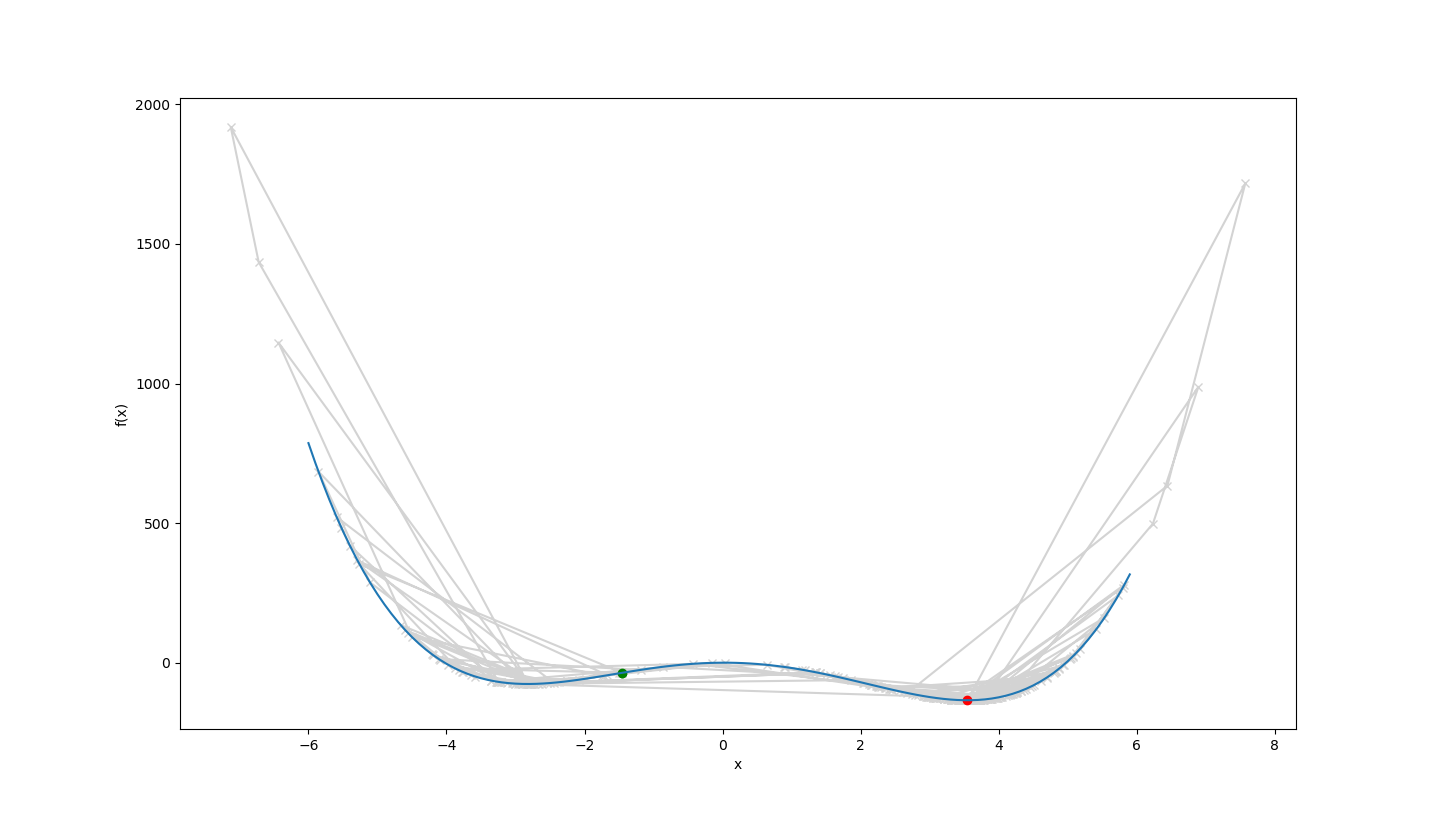
\includegraphics[width=0.8\textwidth]{Q132.png}
\caption{Représentation de l'évolution de l'algorithme (gris), à la surface de $f$ (bleu), le point de départ est indiqué en vert et celui d'arrivée en rouge.}
\label{Q1_T}
\end{figure}

\begin{center}
\fcolorbox{black}{lightgray}{
\begin{minipage}{\linewidth}
\textbf{Remarque sur l'algorithme :} \\
\begin{itemize}
    \item Le point de départ est choisi aléatoirement dans une lois uniforme selon deux bornes données par l'utilisateur.
    \item En plus du critère d'arrêt établi par rapport à un nombre d'itérations, une seconde condition d'arrêt a été établi sur le pourcentage d'acceptation, c'est à dire le nombre de mouvement retenu par rapport au nombre d'itérations total. On peut en effet estimer que si ce pourcentage est faible alors l'algorithme ne conserve que très rarement des solutions, et est donc dans un minimum local de la fonction de coût.\\
    
\end{itemize}
\end{minipage}}
\end{center}
\newpage
\subsection{Fonction de $\mathbb{R}^2$ dans $\mathbb{R}$}
Nous étudions la fonction $g(x,y)= x^4-x^3-20x^2+x+1 +y^4-y^3-20y^2+y+1$; cette fonction a été dans le TD 1 exercice 3; ainsi nous savons qu'elle possède 9 points caractéristique, un maximum local, quatre points selle , et 4 minimum dont un minimum global \textbf{[\ref{Q21}}.
\begin{figure}[H]
\centering
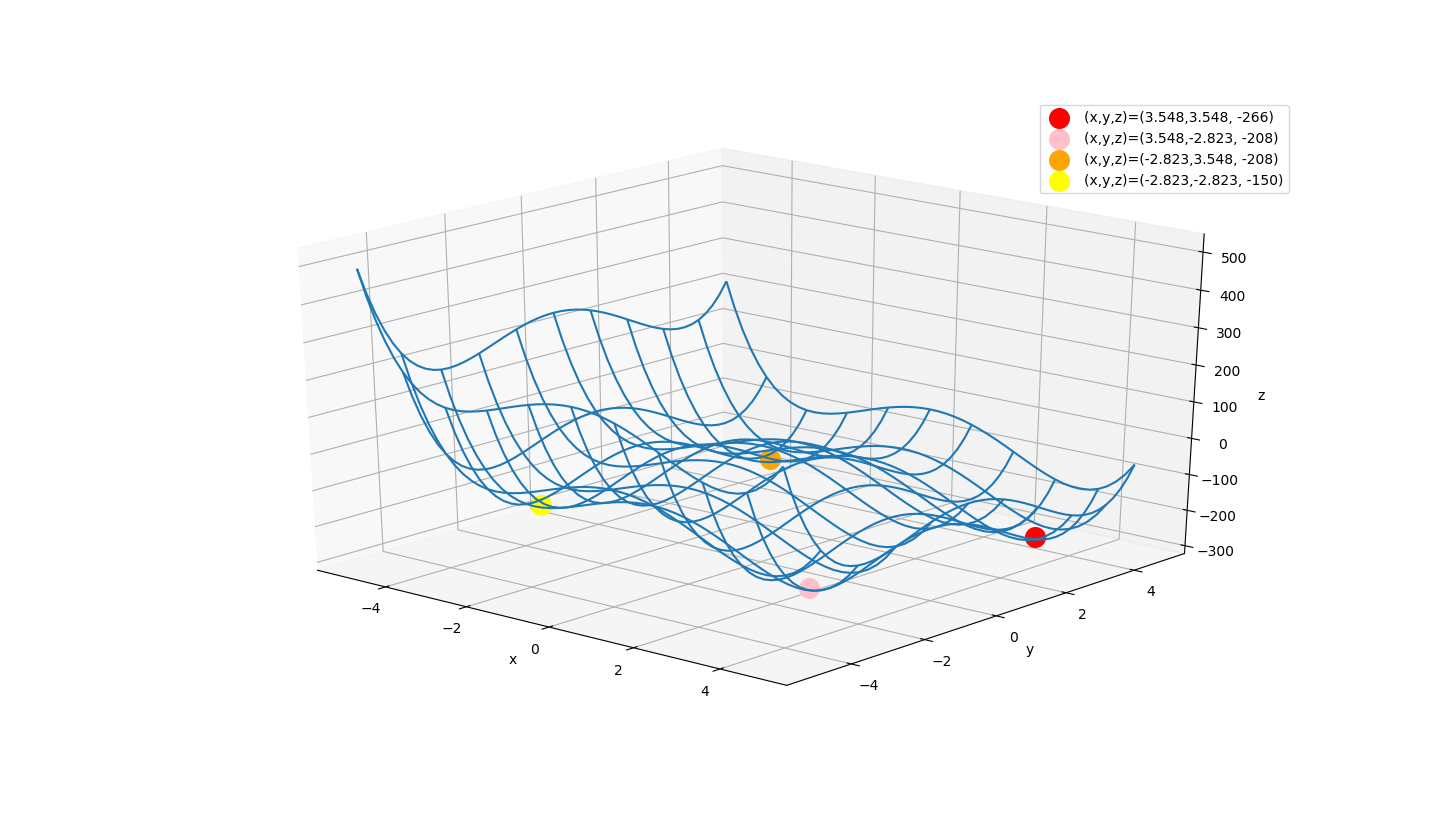
\includegraphics[width=0.8\textwidth]{Q21.png}
\caption{Représentation de la fonction g et de ces quatre minimums, et de leurs coordonnées.}
\label{Q21}
\end{figure}

\begin{minipage}{0.5\textwidth}
Nous reprenons l'analyse des paramètres avec la même stratégie que dans le cas précédent ainsi en fixant $k'=0.5$, $x_0=0$, $y_0=0$ et $t_{max}=10000$ nous faisons varier $k$ tel que $k\in [0,30]$ . Graphiquement il est difficile de conclure sur l'influence du paramètre \textbf{[\ref{Q2K}]}
. Il en est de même en faisant varier $k'$ les autres paramètres restant égaux par ailleurs.
\end{minipage} \hfill
\begin{minipage}{0.45\textwidth}
\begin{figure}[H]
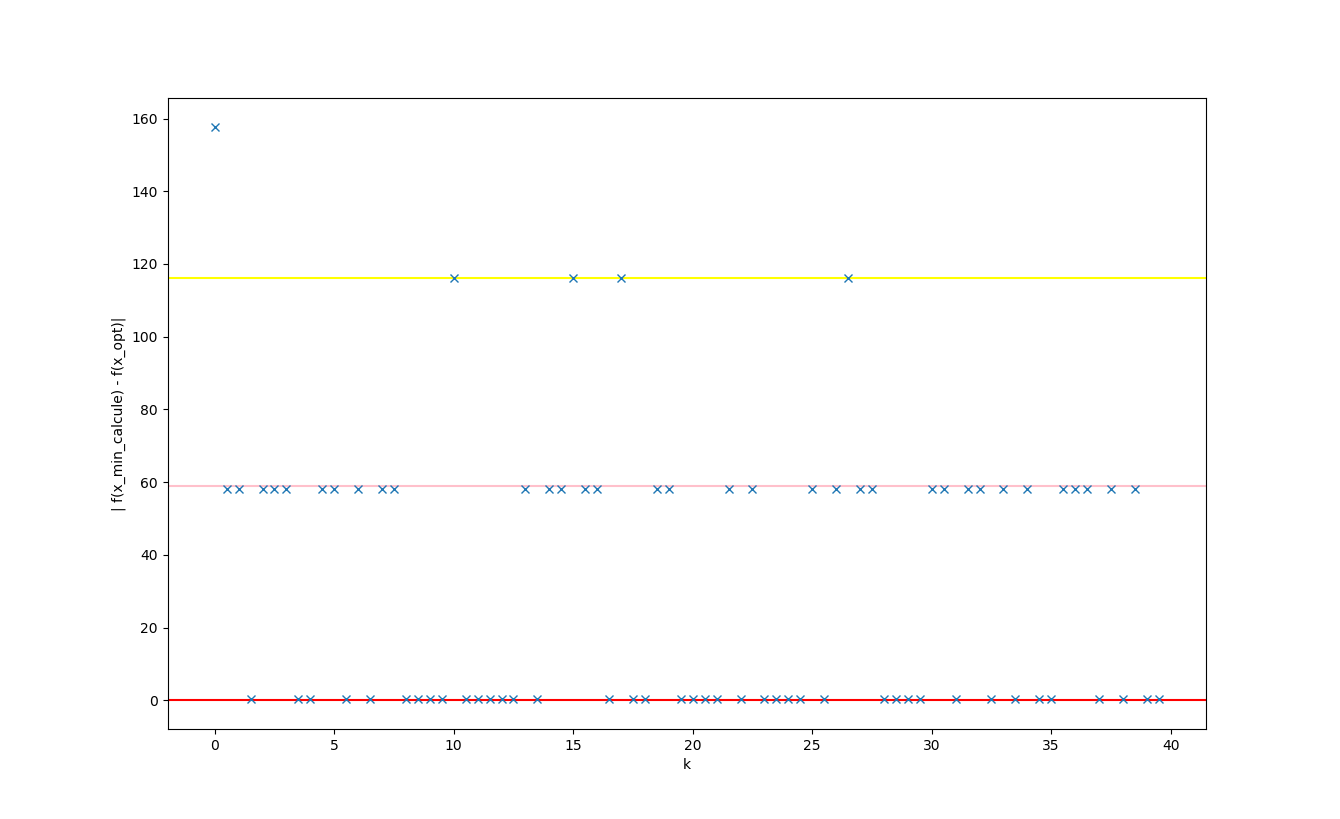
\includegraphics[width=1\textwidth]{Q2K.png}
\caption{Représentation de la fonction g et de ces quatre minimums, et de leurs coordonnées.}
\label{Q2K}
\end{figure}
\end{minipage}
\\
Nous utilisons le test statistique mis en place pour analyser ces résultats :
\begin{itemize}
    \item Pour comprendre l'effet de $k$, nous testons si le nombre de succès est supérieur lorsque k est supérieur à 7.5 par rapport aux situations où k est inférieur à 7.5. Nous trouvons une statistique de 2.079 et une pvalue de  $1e-3$, nous rejetons donc H0 ($H0 : \quad \hat{s}_{k<7.5} =\hat{s}_{k>7.5} \quad;  H1 :\quad \hat{s}_{k<7.5} < \hat{s}_{k>7.5} $).
    \item Pour comprendre l'effet de $k'$, nous testons si le nombre de succès est supérieur lorsque k est inférieur à 0.5 par rapport aux situations où k est inférieur  à 05. Nous trouvons une statistique de 2.23 et une pvalue de  $1e-3$, nous rejetons donc H0 ($H0 : \hat{s}_{k'<0.5} =\hat{s}_{k'>0.5}  \quad;  H1 :\quad \hat{s}_{k<7.5} < \hat{s}_{k>7.5} $).
\end{itemize}


\subsection{Compréhension de l’algorithme}
\textbf{\color{brick}1.} L'algorithme du recuit simulé explore l'espace de façon aléatoire, ce type de recherche du minimum peut être bénéfique lorsque :
\begin{itemize}
    \item la fonction à minimiser n'est pas dérivable,
    \item la fonction à minimiser n'est pas continue,
    \item l'algorithme 'chute' dans un minimum local, il peut le contourner.
\end{itemize}
\vspace{0.5cm}
\textbf{\color{brick}2.} La température intervient deux fois dans l'algorithme du recuit simulé. Une première fois dans le choix d'un $x$ voisin de la position courante avec $X_{t+1}= x_t + N(0, ke^{-1/1000T})$, et une seconde fois dans la probabilité d'accepter un $x$ induisant une augmentation de la fonction de coût. En début de simulation  $T =1$ le voisinage es définit sur un grand espace et la probabilité d'accepter ce voisin est relativement grande, en fin de simulation $T$ est faible alors la recherche de voisins est réalisée dans une surface petite et la probabilité d'acceptation est faible. \\
Par analogie aux processus de recuit en début de processus le niveau d'énergie du système, auquel peut être associé la fonction de coût, est relativement grand, ce niveau d'énergie fluctue ensuite aléatoirement jusqu'à atteindre d'un équilibre thermique. De plus en physique la loi de Bolltzman nous apprend que la probabilité d'observer un système à une énergie donné $E$ est fonction de la température de l'environnement telle que $e^{-E/T}$, ainsi plus la température diminue plus la probabilité d'observer cet état diminue.  \\
En d'autre terme à l'initiation du processus l'algorithme procède à une recherche 'naïve' sans connaissance de l'environnement énergétique, ainsi l'algorithme progresse  par  oscillations, puis l'ampleur de ces oscillations est diminue avec la température. À la fin du processus les oscillations sont quasi nuls ce qui nous permet de conclure à la convergence de l'algorithme.\\
Cependant la convergence vers un minimum global n'est pas garanti, il dépend d'un compromis entre le temps de calcul et le meilleur résultat possible. En effet si la décroissance thermique est trop rapide l'algorithme perd rapidement en 'souplesse' et risque de converger vers un minimum local.\\
\\
\textbf{\color{brick}3.} Comme nous l'avions expliqué $k'$ permet de pondérer la probabilité d'acceptation de voisins induisant une augmentation de la fonction de coût. Plus on diminue $k'$ plus on restreint l'exploration, on pourrait ainsi  augmenter l'efficacité mais ceci dépend de la condition initiale. En étant laxiste envers l'erreur on augmente l'aire explorée mais là encore  on ne garantit pas la convergence vers un minimum global. Il existe une valeur optimale de $k'$.\\
Le paramètre $k$ pondère l'ampleur des oscillation, à l'instar du paramètre $k'$ une augmentation de $k$ accroît l'aire explorée et donne une certaine souplesse à l'algorithme, réciproquement une diminution de $k$ pourrait augmenter la vitesse de convergence à condition d'être dans le voisinage du minimum global.



\end{document}